\lab{Python}{Computer Caches}{Caches}
\objective{Understand the role caches play in computational performance.}

The real computational bottleneck of computers lies in the memory system, not the processor.  
In the early days of computing, memory speed and CPU speed were evenly matched.  
The CPU relatively quickly access data directly from RAM.  
Now, the CPU spends a large amount of time waiting for data to process.  
RAM simply isn't fast enough to keep up.  With CPUs crunching numbers at faster and faster rates, higher performance memory needed to be placed between a relatively slow RAM to cache data.  

\section*{Caching}
Caches were introduced to keep often-used memory accessible very quickly.  High speed memory is very expensive.
There are economical constraints on how much cache is available in a CPU.
Another constraint is efficiency.  The faster the memory cache, the smaller it must be.
Computers have to be able to search all of the cache very quickly.

Caches are effective in two main scenarios: temporal locality and spatial locality.
Temporal locality describes the situation where we reuse specific parts of memory over and over again.
These often-used memory locations are cached so as to make them more quickly accessible.
Spatial locality describes the situation where access memory sequentially in blocks.
We can cache a particular memory address and all the address around it as well.
If we use algorithms that can take advantage of these two data usage patterns, caching will provide a tremendous speed boost.
However, if we are not intelligent in our choice of algorithm, we will be forcing the CPU to sit idle as it waits for data to be fetched from main memory.
The optimal strategy for an efficient algorithm is to fetch sequential blocks of data and reuse them as much as possible before sending it back out to main memory.
For the last few decades, the bottleneck in performance has been memory speed, not processor speed.


\section*{Cache lines}
When data is fetched from caches, it fetches bytes that are around the requested byte.  
If we want to access bytes near the initially requested byte it results in a cache hit.
Requested other values in the same cache line has close to no overhead.
The moment we request a byte outside the cache line, we have to search the cache for it.  If it is not in cache, we have a cache miss.
Bytes are brought into the cache in blocks called \emph{cache lines}.
We can measure the cache line size by stepping through an array with different step sizes.
We have done this in Figure \ref{fig:linesize}.  We are using 32 bit integer arrays in all of our tests.
We start to see a drop in run times after a step size of 16.
Since a 32 bit integer is 4 bytes, we arrive at a cache line size of 64 bytes ($4 \mbox{~bytes} * 16 \mbox{~integers} = 64 \mbox{~bytes}$).
\begin{figure}[h]
\centering
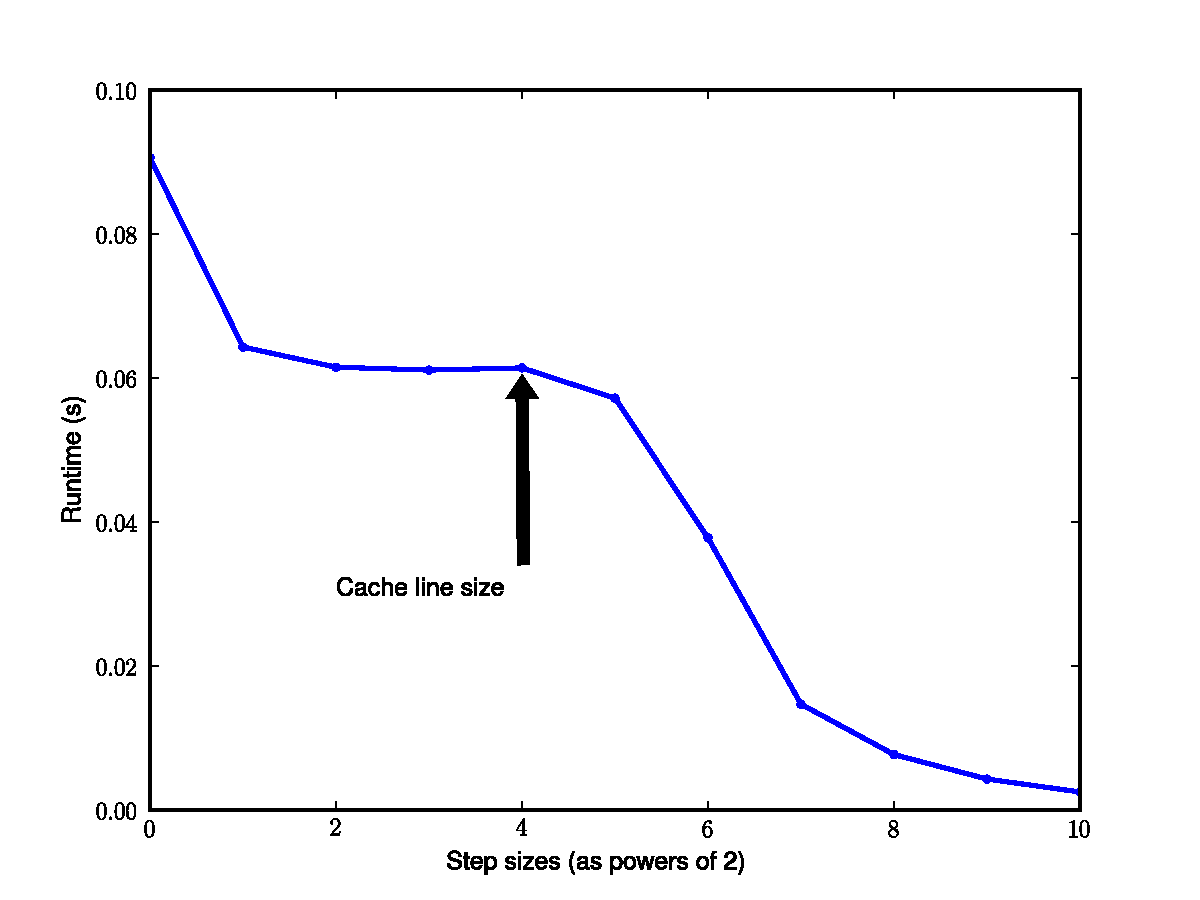
\includegraphics[width=\textwidth]{cache_line.pdf}
\caption{Determining cache line size by looping through a 128MB array with different step sizes.}
\label{fig:linesize}
\end{figure}


\begin{problem}
Find the cache line size for your machine.
To compile you the included C program, you will need a C compiler.
We recommend gcc with the flags \texttt{-O3 -mtune=native}.
The C program expects two arguments: first, the candidate cache line size, and second, the number of loops to run during testing.
The program will print out how many seconds on average one loop took to execute in seconds.
Plot the results of your timings.
\label{prob:cacheline}
\end{problem}

\section*{Cache Size}
Various levels of caches were inserted between main memory and the CPU.  
As cache sizes grow, their access times slow down.
Level 1 (L1) cache was wired directly into the processor.  Level 2 (L2) cache was wired directly into the motherboard.  
Many multi-core processors these days have a third (L3) cache in addition to L1 and L2 caches.  
L1 cache is smallest cache at around 32 kilobytes with the fastest with access times of around 1 nanosecond.  
L2 cache comes in at about 3 nanoseconds.  L3, the largest, but slowest of the caches, clocks in at about 10 to 20 nanoseconds. 
Main memory finally takes about 100 nanoseconds to access.  L2 caches are typically a few hundred kilobytes for modern processors. 
L3 cache, if present, is generally the largest of the caches with sizes ranging between 1 to 20 megabytes. 
RAM is typically several gigabytes.  If your processor has multiple cores, each core usually has its own separate L1 and L2 caches and share an L3 cache with other other cores.

We can measure the drops in performance that occur when we overflow the cache (Figure \ref{fig:cachesizes}).
We performed measurements on an Intel i7-2640M processor.  The cache line size is 64 bytes.
\begin{figure}[h]
\centering
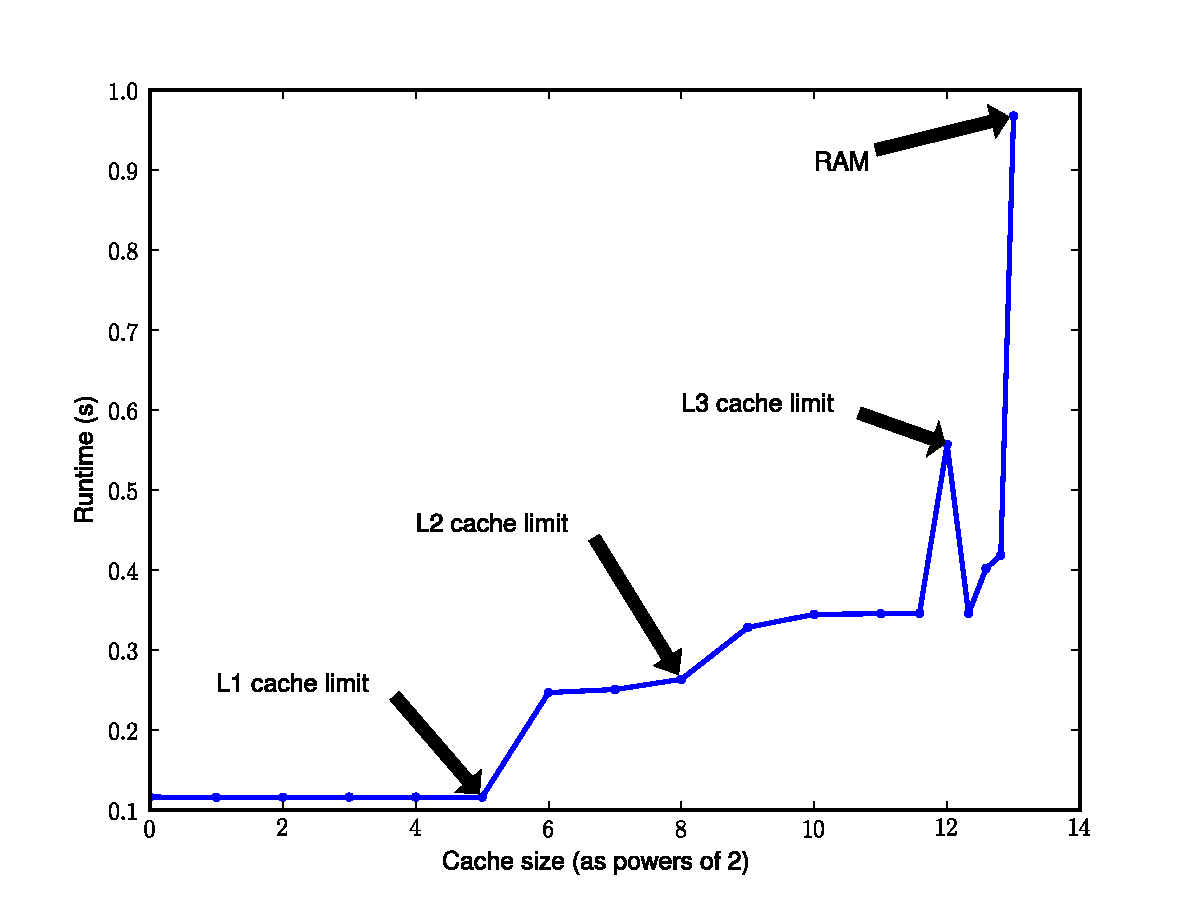
\includegraphics[width=\textwidth]{cache_size.pdf}
\caption{The increases in runtime occur at 32KB, 256KB and 4MB which correspond to the sizes of L1, L2, and L3 caches.}
\label{fig:cachesizes}
\end{figure}

\begin{problem}
Measure the size of your L1 and L2 caches using the cache line value obtained in
Problem \ref{prob:cacheline}.  
To compile you the included C program, you will need a C compiler.
We recommend gcc with the flags \texttt{-O3 -mtune=native}.
The C program expects three arguments: first, the candidate array size, second, the cache line size, and third, the number of loops to run during testing.
The program will print out how many seconds on average one loop took to execute in seconds.
Plot the results of your measurements.
\end{problem}

\section*{Solutions to CPU Starving}
\emph{CPU starvation} refers to the condition of have to wait a relatively long time data to compute.
The way to solve the CPU starvation problem is to be aware of how your data is laid out in memory.
NumPy has support for two main types of memory layouts for arrays.
\begin{description}
\item[Row-major:] Arrays are stored by rows in continuous memory.
Languages such as C and Python use row-major indexing.  NumPy arrays by default use this indexing convention.
Slicing down columns is slow.  In NumPy, row-major arrays are identified as \emph{C contiguous} (\li{order=`C'}).
\item[Column-major:] Arrays are stored by columns in contiguous memory.
Languages like FORTRAN, MATLAB, and R use column-major indexing.  Slicing across rows is slow.
In NumPy, column-major arrays are identified as \emph{FORTRAN contiguous} (\li{order=`F'}).
\end{description}
Paying attention to how your arrays are indexed will be beneficial to the performance of your algorithms.
Some algorithms work better with one type of indexing

While NumPy is very fast for most purposes, it has a tendency to create many temporary arrays as it evaluates results.
The code below will result in the creation of many different arrays, each the size of \li{x}!  
Calculating $y$ takes about one second on the author's machine.
\begin{lstlisting}
x = np.linspace(-1, 1, 10*1024*1024)
y = 1.25*x**3 - .33*x**2 + .75*x + 1.2
\end{lstlisting}
We can reduce the runtime by using a little bit of algebra.
Factoring the expression results results in a much easier expression for the computer to evaluate.
Calculating the equivalent expression takes $.146$ seconds!
\begin{lstlisting}
y = ((1.25*x - .33)*x + .75)*x + 1.2
\end{lstlisting}
A tremendous speed up for not a whole lot of work.

Numexpr, a library for python, is designed to utilize the CPU cache as well as avoid unnecessary temporary arrays.
It evaluates the following expression allocating only a single array and operating on $x$ in blocks that fit into the CPU cache.
It calculates the entire expression for that particular block, then saves the result.
One the authors machine, numexpr executed the unfactored expression in $.0387$ seconds and the factored expression in $.0349$ seconds. 
\begin{lstlisting}
import numexpr as ne
yne = ne.evaluate('1.25*x**3 - .33*x**2 + .75*x + 1.2')
\end{lstlisting}
Using numexpr instead of NumPy can speed up simple vector computations significantly.
These large gains in performance are primarily for large arrays.  
Numexpr will operate on these large arrays in blocks that fit into the CPU cache.  
Numexpr is also designed to easily take advantage of multiple cores by default, a feature that NumPy lacks.
The above evaluations using numexpr we done using 4 threads.  
Please refer to the numexpr Users Guide (\url{https://code.google.com/p/numexpr/wiki/UsersGuide}) for information on what operations are supported by numexpr.
